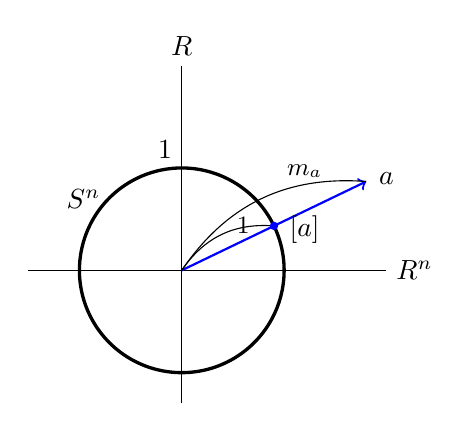
\begin{tikzpicture}[scale=1.3]
  % draw axes
  \draw (0, -1.3) -- (0, 2) node[anchor=south]{$\mathbb{R}$};
  \draw (-1.5,0) -- (2,0) node[anchor=west]{$\mathbb{R}^n$};

  \draw (0,1) node[anchor=south east]{$1$};

  % plot
  \draw[very thick, domain=0:360, smooth, variable=\t, samples=100] 
    plot ({cos(\t)}, {sin(\t)});

  \draw (-0.7, 0.7) node[anchor=east]{$\mathbb{S}^n$};

  \draw[blue, thick, ->, trig format=rad] (0,0) -- ({2*cos(pi/7)}, {2*sin(pi/7)});

  \draw (0,0) to [bend left=30] ({cos(deg(pi/7))}, {sin(deg(pi/7))});
  \draw (0.6,{sin(deg(pi/7))}) node {\small $1$};

  \draw (0,0) to [bend left=30] ({2*cos(deg(pi/7))}, {2*sin(deg(pi/7))});
  \draw (1.2,{2*sin(deg(pi/7))+0.1}) node {\small $m_{\vc a}$};

  \filldraw[blue] ({cos(deg(pi/7))}, {sin(deg(pi/7))}) circle (1pt);
  \draw (2, 0.9) node { $\vc a$};
  \draw (1.2, 0.4) node { $[\vc a]$};
\end{tikzpicture}
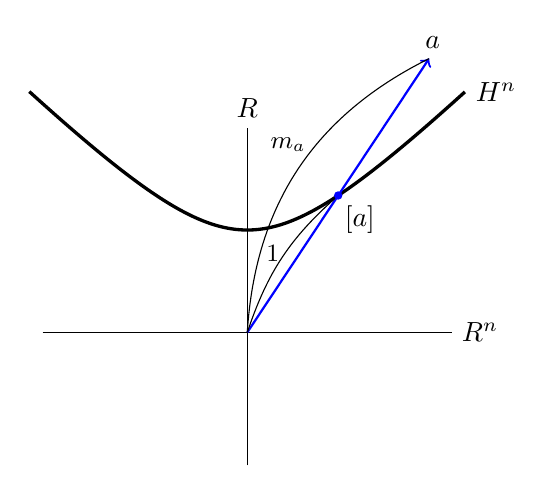
\begin{tikzpicture}[scale=1.3]
  % draw axes
  \draw (0, -1.3) -- (0, 2) node[anchor=south]{$\mathbb{R}$};
  \draw (-2,0) -- (2,0) node[anchor=west]{$\mathbb{R}^n$};

  \draw[very thick, domain=-1.5:1.5, smooth, variable=\t, samples=100] 
    plot ({sinh(\t)}, {cosh(\t)}) node[anchor=west]{$\mathbb{H}^n$};
  % \draw[domain=-1.5:2, smooth, variable=\x] plot ({\x}, {\x});
  % \draw[domain=-2:1.5, smooth, variable=\x] plot ({\x}, {-\x});

  \draw[blue, thick, ->, trig format=rad] (0,0) -- ({2*sinh(0.8)}, {2*cosh(0.8)});

  \draw (0,0) to [bend left=15] ({sinh(0.8)}, {cosh(0.8)});
  \draw (0.25,{0.5*cosh(0.8)+0.1}) node {\small $1$};

  \draw (0,0) to [bend left=30] ({2*sinh(0.8)}, {2*cosh(0.8)});
  \draw (0.4,{cosh(0.8)+0.5}) node {\small $m_{\vc a}$};

  \draw ({2*sinh(0.75)}, {2*cosh(0.8)}) node[anchor=south west] { $\vc a$};
  \filldraw[blue] ({sinh(0.8)}, {cosh(0.8)}) circle (1pt);
  \draw (1.1, 1.1) node { $[\vc a]$};
\end{tikzpicture}
